\chapter{Hydration free energy}

\section{Introduction}
%
In this example, we seek to compute the relative hydration free energies of different ligands in explicit solvent.
%
We will use the approach of transdimensional nonequilibrium switching to compute relative hydration free energies for a set of molecules in the FreeSolv dataset~\cite{Mobley2014,DuarteRamosMatos2017}, a set of experimentally and computationally characterized hydration free energies for small molecules.
%
Although this is a simple test, it demonstrates that the algorithm is capable of efficiently producing low-variance work values in explicit solvent, and among diverse sets of ligands.
%
For the example presented in this chapter, we will be using a randomly selected subset of substituted benzene molecules.
%
For each pair of ligands, we will run 1 nanosecond of equilibrium simulation and a nonequilibrium switching protocol 5 picoseconds long. 
%
We will use 1000 switching trajectories in the forward and reverse direction for each pair, and then use the work values to estimate the relative free energies.
%
\section{Thermodynamic Cycle}
%
In order to compute the relative hydration free energy, we employ a thermodynamic cycle wherein we transform the small molecule from one molecule to another in solvent and in vacuum, and subtract the resulting free energies, depicted in \ref{fig:thermocycle}.
%
\begin{figure}
    \centering
    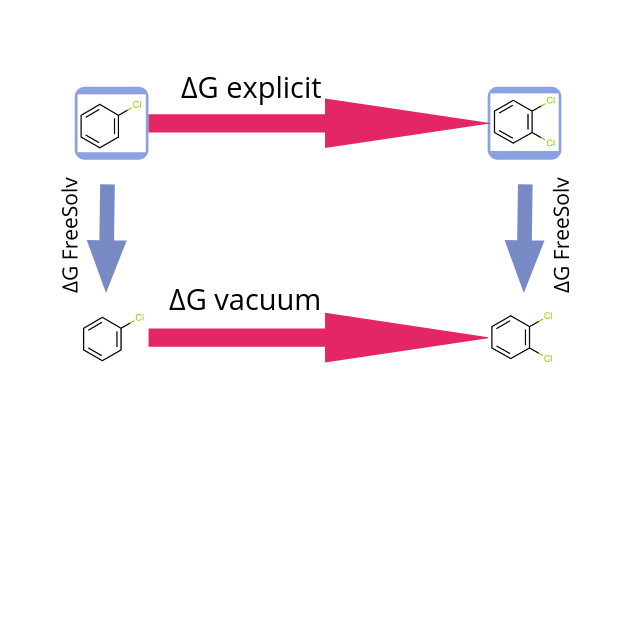
\includegraphics[width=1.0\textwidth]{thermocycle.png}
    \caption{The thermodynamic cycle of the hydration free energy calculation. Blue arrows denote the data available in FreeSolv; magenta arrows denote the legs performed in this work.}
    \label{fig:thermocycle}
\end{figure}
%
We compare to FreeSolv~\cite{Mobley2014}, which is a database of computed absolute hydration free energies; therefore, in order to compare our results to FreeSolv, we will need to compute relative hydration free energies from the absolute data.
%
\section{Vacuum Phase}
%
For the vacuum phase of the simulation, we performed 1 ns of equilibrium simulation for each molecule, and 100 switches between each pair in both directions.
%
For the nonequilibrium switching length, we used 5ps, as it was sufficient for explicit solvent, and so should be sufficient for vacuum.
%
%
\subsection{Explicit Phase}
%
\subsection{Nonequilibrium switching protocol length}
%
Prior to performing this calculation, we performed a quick check of the performance of various nonequilibrium switching times vs. the amount of work that was performed.
%
In this check, we simulated benzene and naphthalene in solvent for 1 nanonsecond, and then performed 100 switching trajectories in each direction.
%
We collected the data and analyzed the standard deviation of the work performed by the protocol, shown in Figure~\ref{fig:benz_naph_protocol_work}
%
\begin{figure}
    \centering
    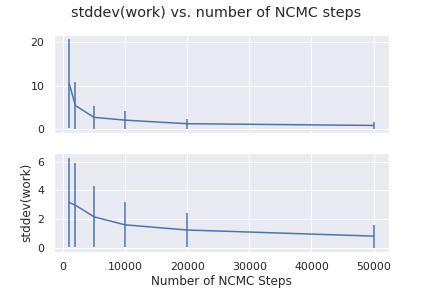
\includegraphics[width=1.0\textwidth]{benz_naph_work_vs_steps.png}
    \caption{The standard deviation of the work for an NCMC switching trajectory between benzene and naphthalene vs. number of steps, with a 1fs timestep. Top: work for transforming benzene into naphthalene. Bottom: work for transforming naphthalene into benzene.}
    \label{fig:benz_naph_protocol_work}
\end{figure}
%
Given that the transformation from benzene to naphthalene is rather difficult without extra bond and angle softening, we decided to use a switching time of 5~picoseconds, and 1000 switching attempts between each pair in each direction.
%
\section{Analysis of the work of the entire move}
%
In addition to the protocol work, we can also examine the distributions of the work of the entire move in both directions.
%
Since this is the quantity that is fed into BAR, it is critical to examine.
%
In \ref{fig:worka}, there is a representative pair of work distributions.
%
\begin{figure}
    \centering
    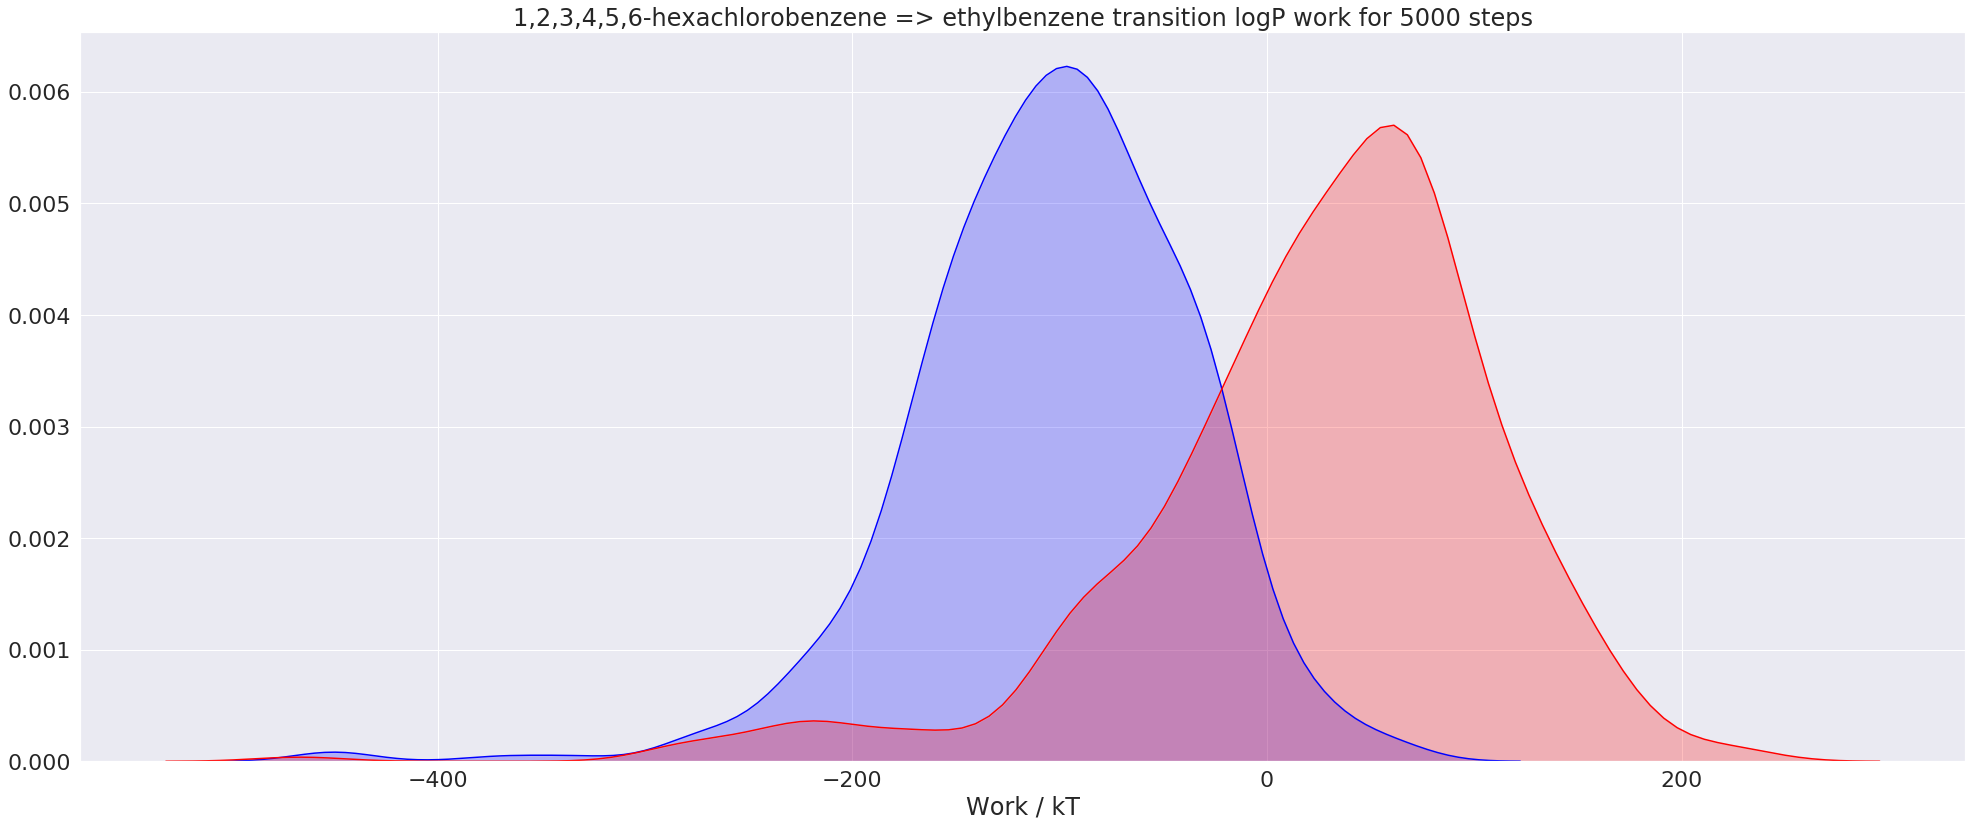
\includegraphics[width=1.0\textwidth]{hexachlor-ethylbenz.png}
    \caption{The forward and reverse (blue and red, respectively) log acceptance probability distributions for transitions between hexachlorobenzene and ethylbenzene. Although the variances of the distributions appear high, the overlap is very good, allowing a low-error free energy estimate.}
    \label{fig:worka}
\end{figure}
%
%
Once again, there appears to be sufficient overlap for proceeding with the estimation of free energy differences.
%
Surprisingly, even in \ref{fig:workb}, the overlap is quite good.
%
\begin{figure}
    \centering
    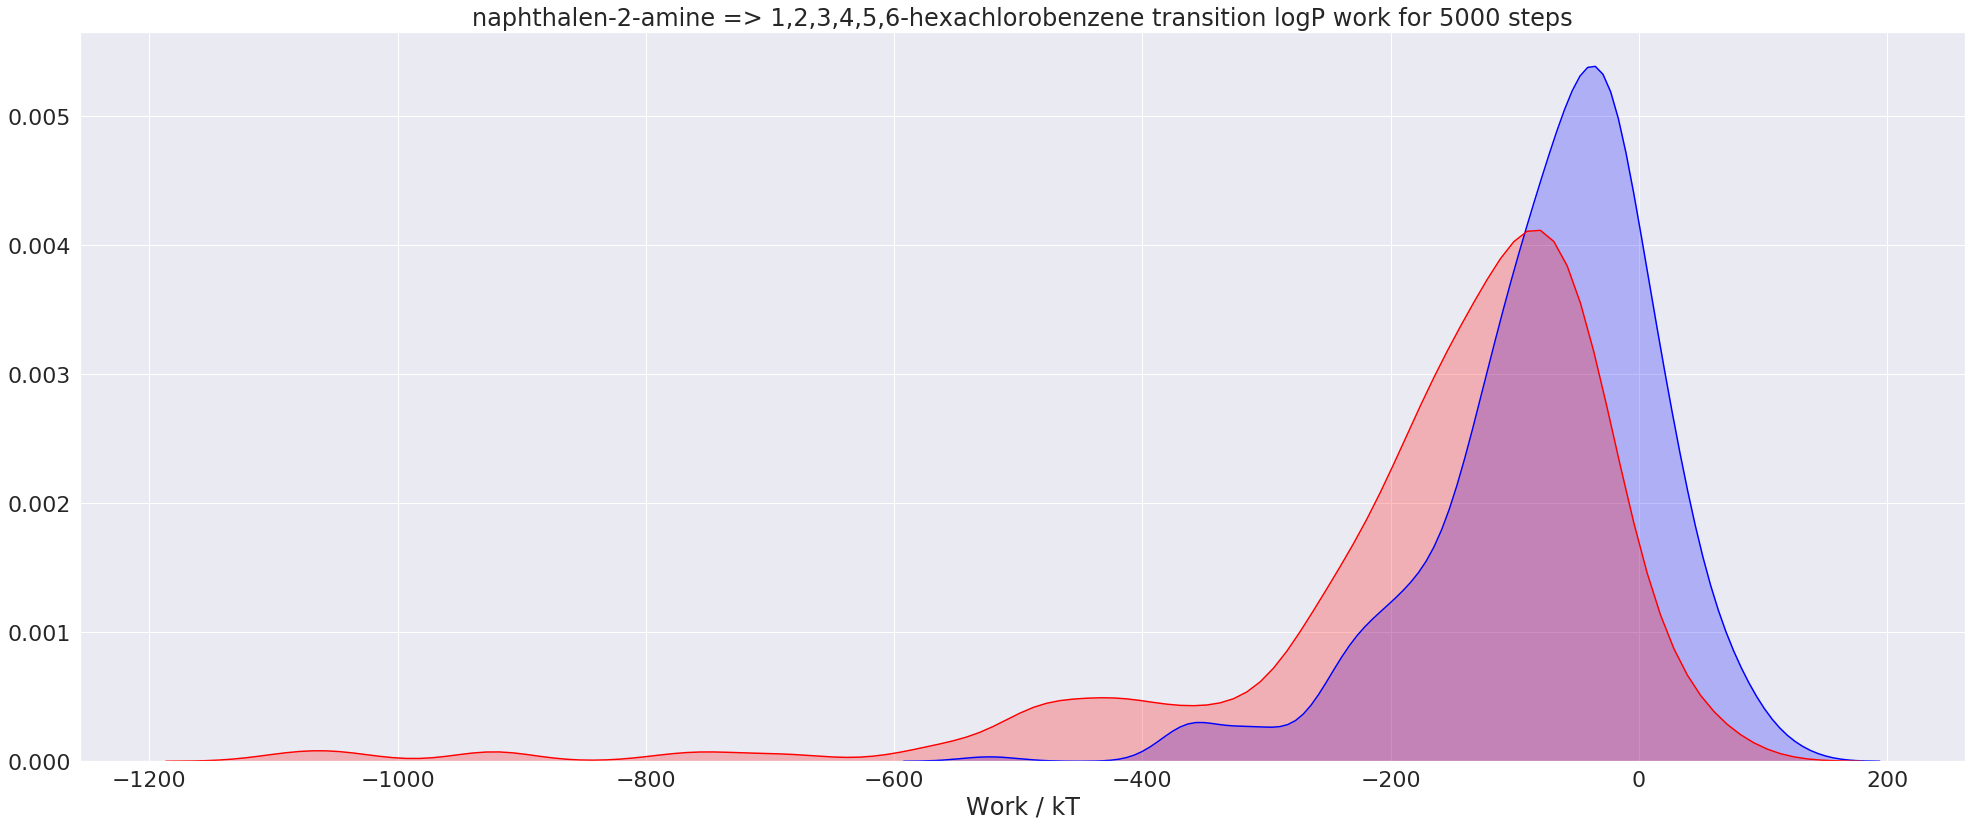
\includegraphics[width=1.0\textwidth]{napthamine-hexachlor.png}
    \caption{The forward and reverse (blue and red, respectively) log acceptance probability distributions for transformations between napthalene-2-amine and hexachlorobenzene. Despite having to create or break a fused ring, the overlap is still quite good, allowing low variance free energy estimates}
    \label{fig:workb}
\end{figure}
%
